\renewcommand{\FileName}{twoway}
% slide template
\begin{frame}
  \frametitle{Two-way frequency tables}
\input{tab/hair-eye}

\begin{itemize}
 \item With a $\chi^2$ test (\PROC{FREQ}) we can tell that hair-color and eye-color are associated.
 \item The more important problem is to understand \alert{how} they are associated.
 \item Some graphical methods:
	\begin{itemize*}
		\item Sieve diagrams
		\item Agreement charts (for square tables)
		\item Mosaic displays
	\end{itemize*}
\end{itemize}
\end{frame}

\subsection{Sieve diagrams}
\begin{frame}
  \frametitle{Two-way frequency tables: Sieve diagrams}
  \begin{itemize}
	\item{\large\bfseries count $\sim$ area}
      \begin{itemize*}
	  \item When row/col variables are independent, $n_{ij} \approx \hat{m}_{ij} \sim n_{i+}
	  n_{+j}$
	  \item $\Rightarrow$ each cell can be represented as a rectangle,
	  with area = height $\times$ width $\sim$ frequency, $n_{ij}$ (under independence)
	  \end{itemize*}
  \end{itemize}
% 	  \begin{center}
% 	  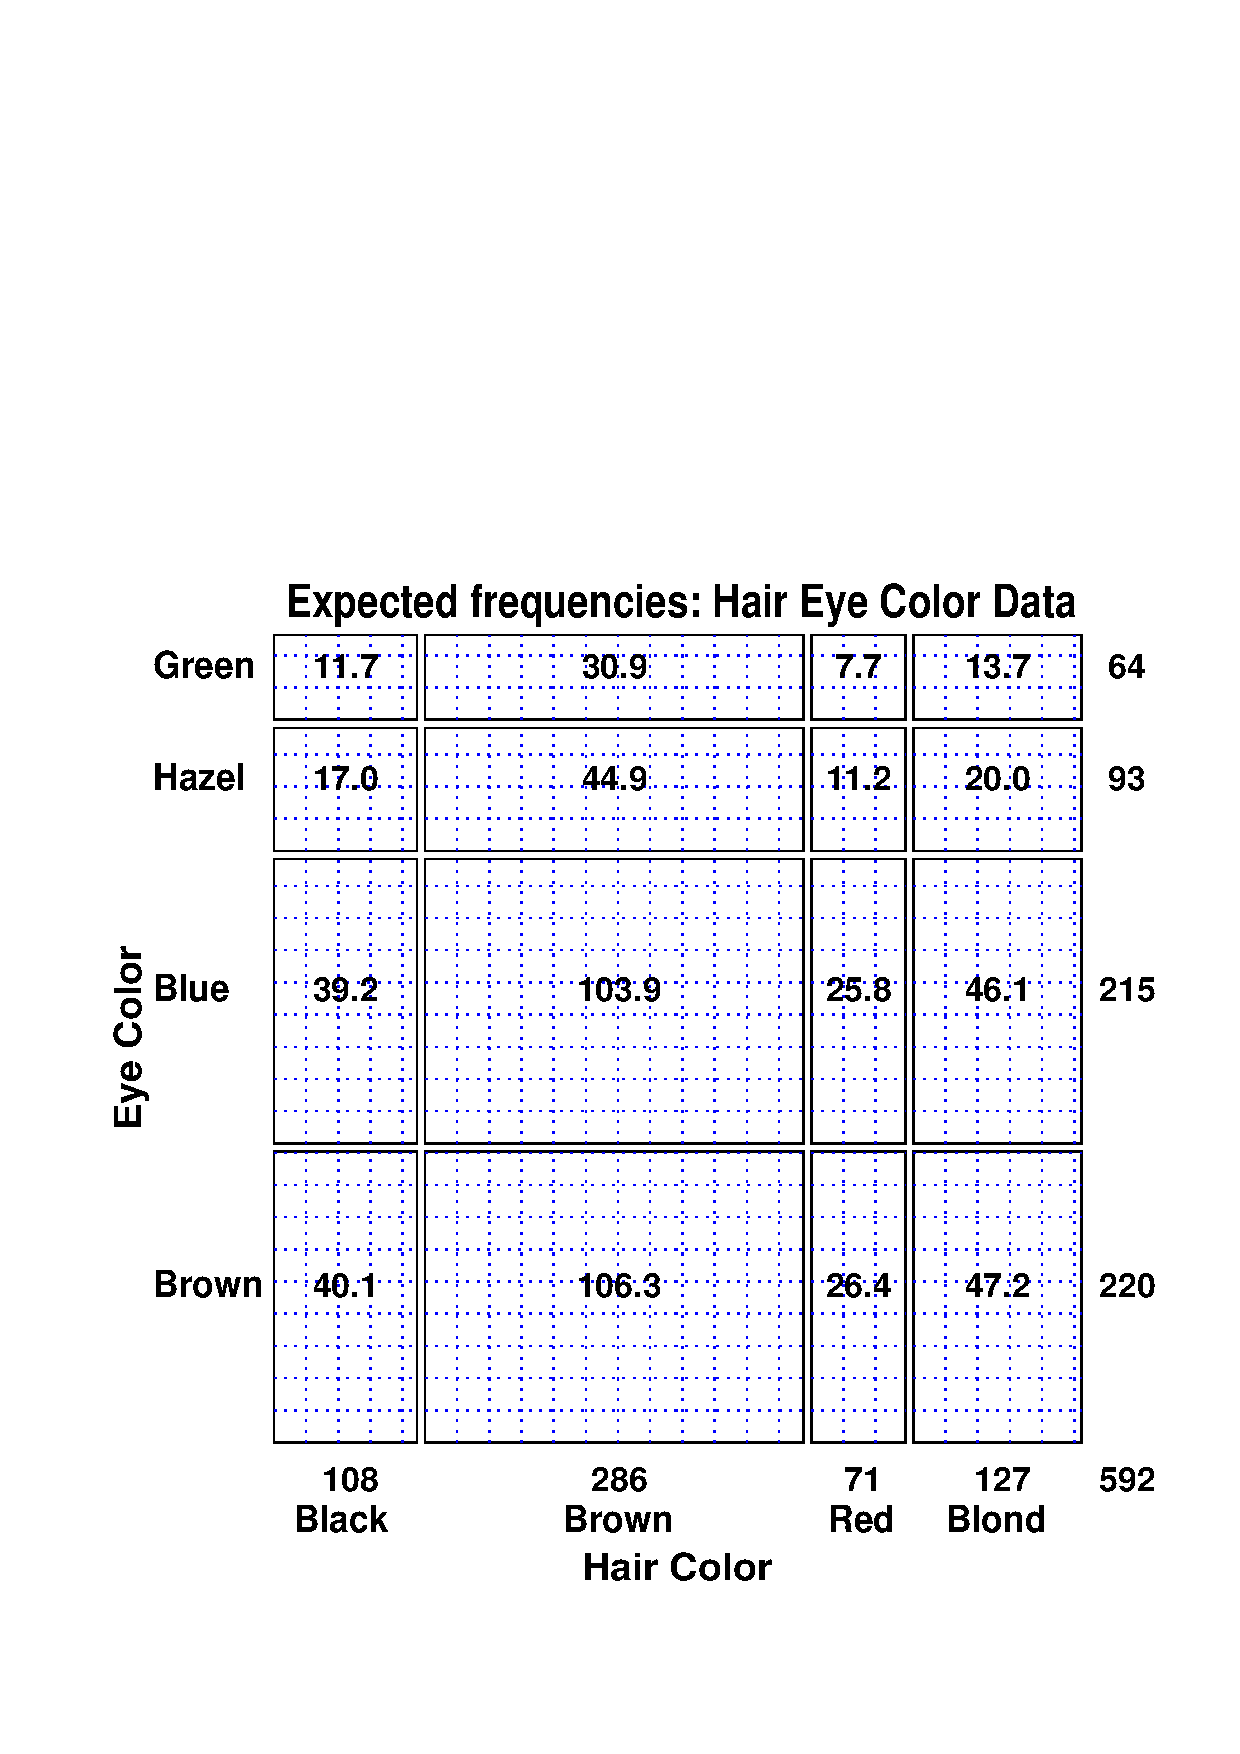
\includegraphics[width=.65\textwidth,clip]{fig/sieve0}
% 	  \end{center}
 \begin{columns}
   \begin{column}{.5\textwidth}
	  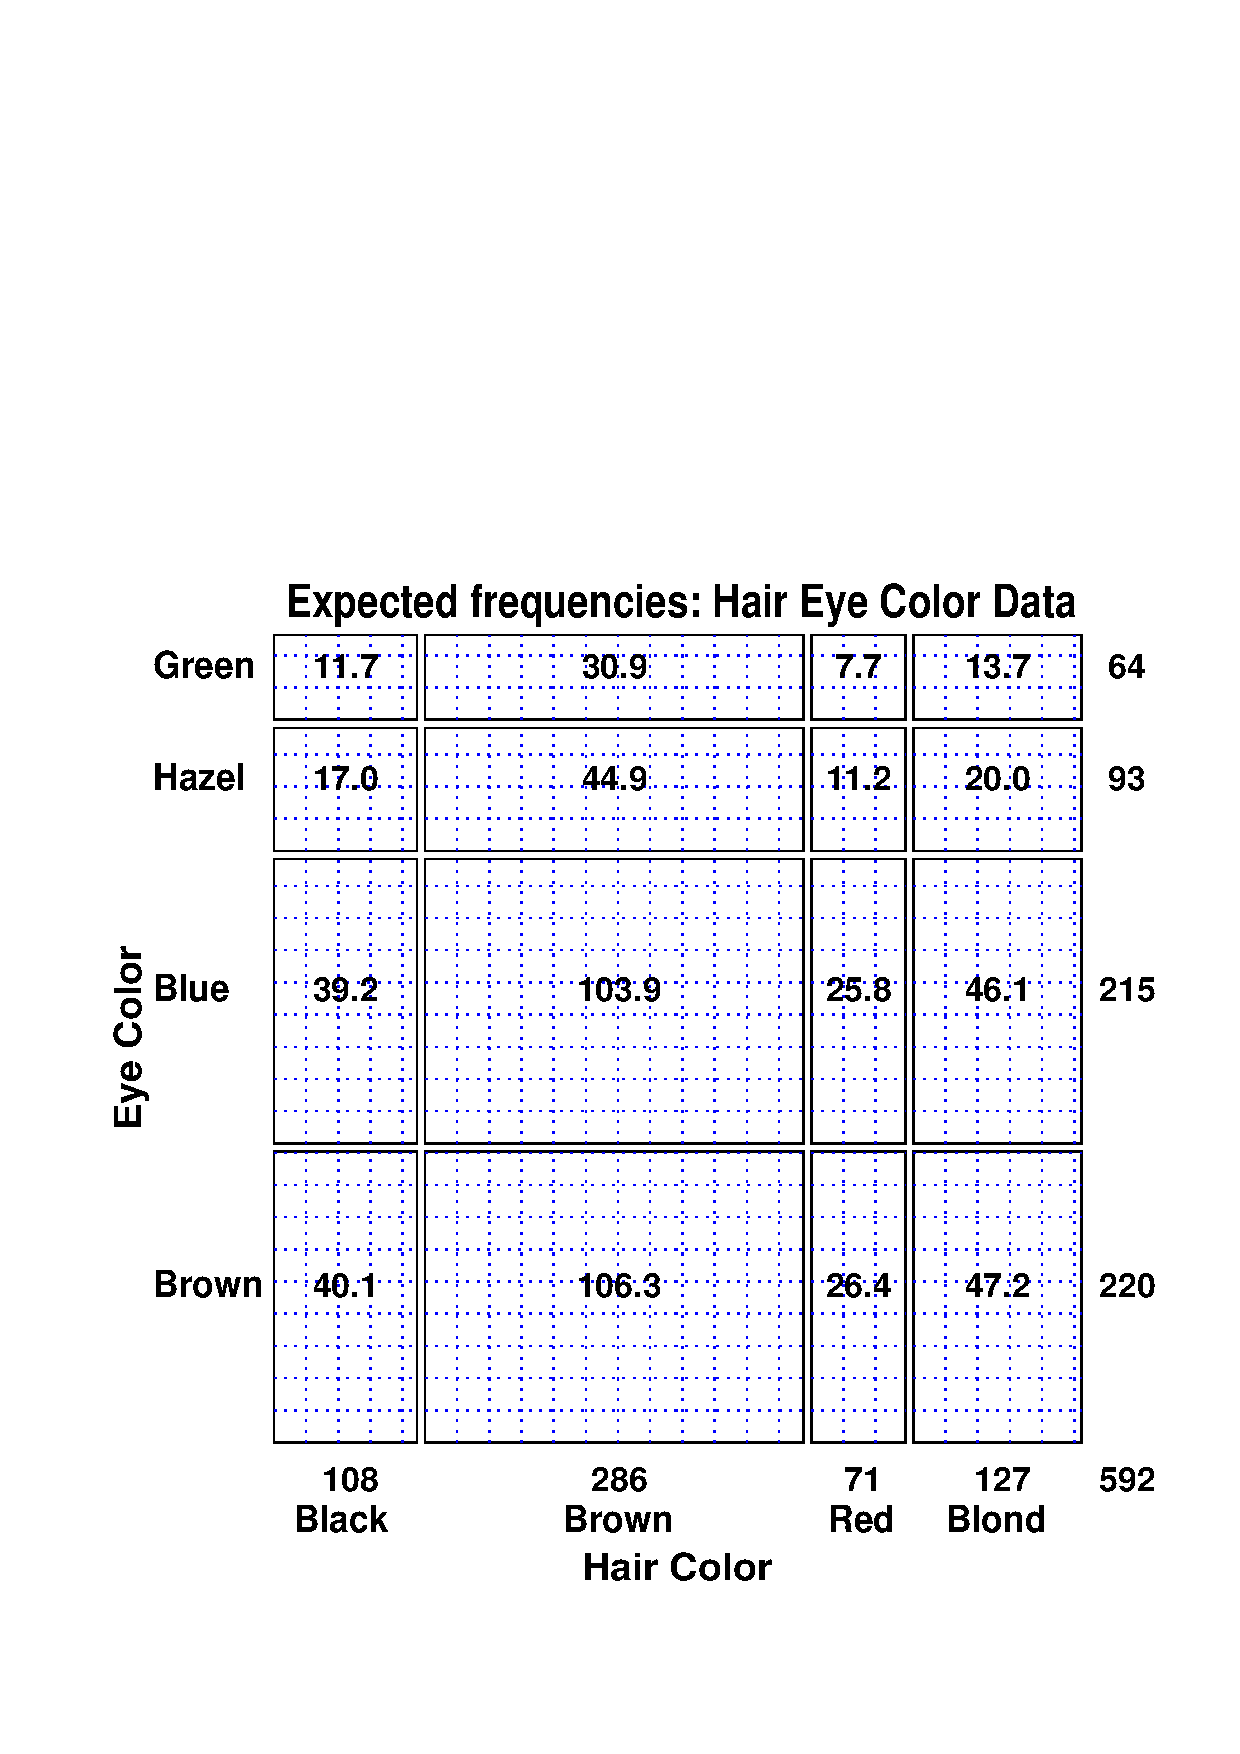
\includegraphics[width=\linewidth,clip]{fig/sieve0}
   \end{column}
   \begin{column}{.5\textwidth}
      \begin{itemize}
       \item This display shows \alert{expected frequencies}, assuming independence, as \# boxes within each cell
       \item The boxes are all of the same size (equal density)
       \item Real sieve diagrams use \# boxes = \alert{observed frequencies}, $n_{ij}$
      \end{itemize}

	
   \end{column}
 \end{columns}

\end{frame}

\begin{frame}
  \frametitle{Sieve diagrams}
  \begin{itemize*}
	\item Height/width $\sim$ marginal frequencies, $n_{i+}$,
	 $ n_{+j}$
	\item Area $\sim$ expected frequency, $\hat{m}_{ij} \sim n_{i+}
	  n_{+j}$
	\item Shading $\sim$ observed frequency, $n_{ij}$, \blue{color}: sign$(n_{ij} -
	\hat{m}_{ij})$.
	\item \boldital{Independence}: Shown when density of shading is uniform.
  \end{itemize*}
	  \vspace{0.5ex}
	  \begin{center}
	  \includegraphics[width=.5\textwidth,clip]{fig/sieve1a1}
	  \end{center}
\end{frame}

\begin{frame}
  \frametitle{Sieve diagrams}
  \begin{itemize*}
	\item {\large\bfseries Effect ordering}: Reorder rows/cols to make the
	pattern coherent
  \end{itemize*}
	  \vspace{1ex}
	  \begin{center}
	  \includegraphics[width=.6\textwidth,clip]{fig/sieve1a2}
	  \end{center}
\end{frame}

\begin{frame}
  \frametitle{Sieve diagrams}
  \begin{itemize*}
	\item Vision classification data for 7477 women
  \end{itemize*}
	  \vspace{1ex}
	  \begin{center}
	  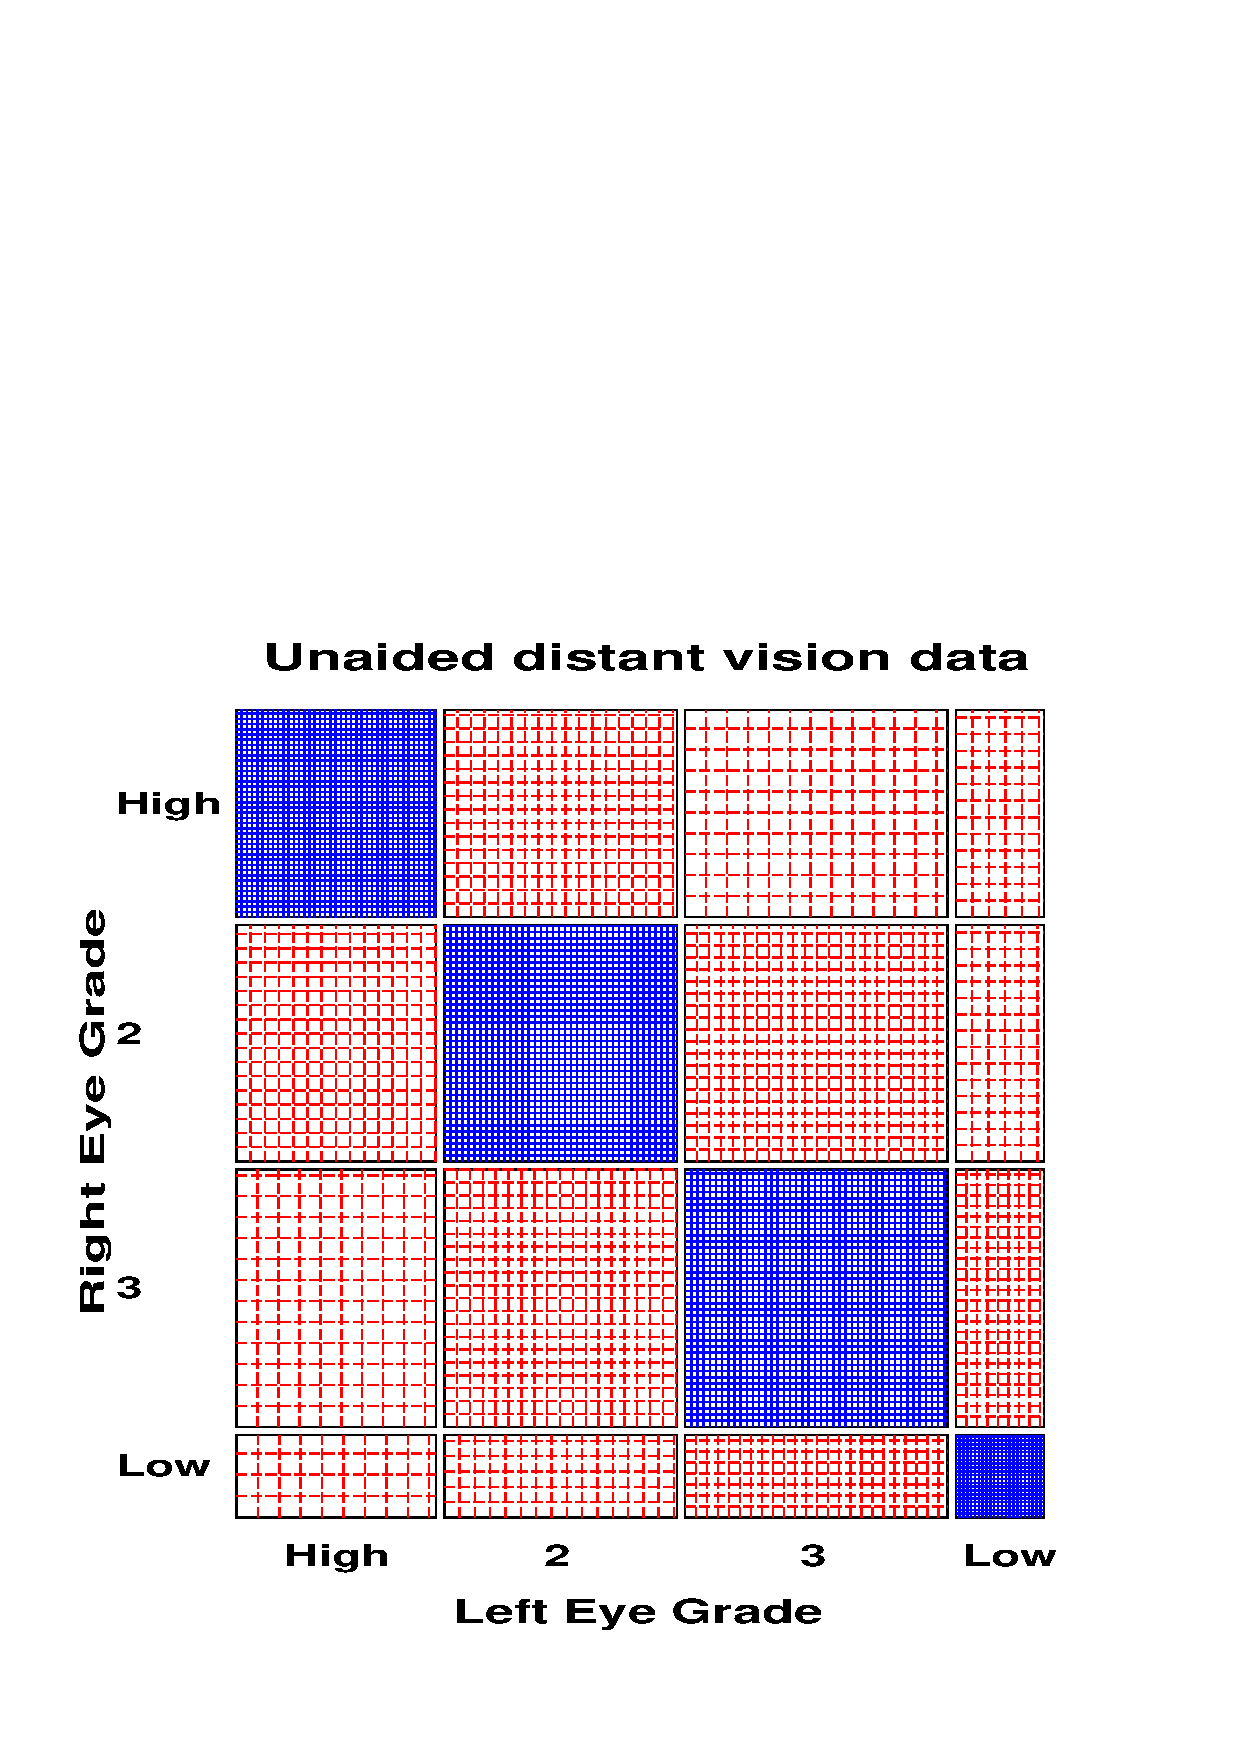
\includegraphics[width=.6\textwidth,clip]{fig/sieve2}
	  \end{center}
\end{frame}

\begin{comment}
\begin{frame}[fragile]
  \frametitle{Sieve diagrams: SAS Example}
\begin{Input}[fontsize=\small,label=\fbox{\texttt{sieve2.sas}},baselinestretch=0.8]
proc iml;
  %include iml(sieve);
    \sascomment{*-- frequency table;}
  tab = \{1520   266   124    66,
          234  1512   432    78,
          117   362  1772   205,
           36    82   179   492 \};
    \sascomment{*-- variable and level names;}
  vnames = \{'Right Eye Grade' 'Left Eye Grade'\};
  lnames = \{ 'High' '2' '3' 'Low',
             'High' '2' '3' 'Low'\};
  title  = \{'Unaided distant vision data'\};
    \sascomment{*-- Global options;}
  \sasemph{run sieve(tab, vnames, lnames, title );}
quit;
\end{Input} 
Online weblet: \url{http://datavis.ca/online/sieve/}
\end{frame}
\end{comment}

\begin{frame}[fragile]
  \frametitle{Sieve diagrams: SAS Example}
\begin{Input}[fontsize=\small,label=\fbox{\texttt{sievem.sas}},baselinestretch=0.8]
data vision;
  do Left='High', '2', '3', 'Low';
  	do Right='High', '2', '3', 'Low';
        input count @@; output;
        end;
    end;
  label left='Left Eye Grade'  right='Right Eye Grade';
datalines;
       1520   266   124    66
        234  1512   432    78
        117   362  1772   205
         36    82   179   492 
;
%sieveplot(data=vision, var=Left Right,
    title=Unaided distant vision data);
\end{Input} 
Online weblet: \url{http://datavis.ca/online/sieve/}
\end{frame}

\begin{frame}[fragile]
  \frametitle{Sieve diagrams: n-way tables in R}
\begin{Rin}
> sieve(UCBAdmissions, sievetype='expected')
\end{Rin}
	  \begin{center}
	  \includegraphics[width=.6\textwidth,clip]{fig/berkeley-sieve1}
	  \end{center}

\end{frame}

\begin{frame}[fragile]
  \frametitle{Sieve diagrams: n-way tables in R}
\begin{Rin}
> sieve(UCBAdmissions, shade=TRUE)
\end{Rin}
	  \begin{center}
	  \includegraphics[width=.6\textwidth,clip]{fig/berkeley-sieve2}
	  \end{center}

\end{frame}
